\chapter{Article 2 - Moment d’apparition des gènes impliqués dans une voie de transduction du signal humaine}
\thispagestyle{firstpage}
\onehalfspacing

\section{Contexte de l'étude}
\par Un des piliers majeurs de l’évolution est la naissance de nouveaux gènes, et elle est en partie due aux duplications de gènes et de génomes. Deux duplications de génomes complets (WGD) sont survenues à la racine des vertébrés lors de la scission avec les invertébrés. De plus, le clade des téléostéens a subi une 3$\textsuperscript{ème}$ duplication de génome complet, et une partie de ces espèces (les salmonidés et les carpes) une 4$\textsuperscript{ème}$. Les périodes de duplications de génome sont suivies de pertes massives de gènes dupliqués. Le clade des téléostéens est donc un modèle de choix pour étudier la capacité de ces gènes à rester à l’état de gènes dupliqués ou leur retour sous forme de singleton. Cette étude est présentée sous forme de schéma récapitulatif en Figure ~\ref{fig:15_schéma2} page ~\pageref{fig:15_schéma2} et est suivie d’un article (page \pageref{art2}) publié dans le journal Heliyon : \parencite{picolo_genes_2021}.

\section{Matériels et méthode}
\par Pour cette étude, nous avons récupéré un ensemble de 2 298 gènes uniques impliqués dans 47 voies de signalisation humaine dans la base de données KEGG V104. Les voies et leurs caractéristiques sont présentées dans le Tableau \ref{table:voiecaracteristiq}.  
\par Afin de déterminer la quantité d’orthologues téléostéens pour chacun de nos gènes impliqués dans une voie de signalisation, nous avons récupéré l’ensemble des orthologues téléostéens par la plateforme Biomart d’Ensembl V107. L’ensemble des espèces de téléostéens dont le génome annoté est disponible sur Ensembl a été utilisé, soit 63 espèces, dont 54 espèces ayant subi 3 duplications de génome complet, et 9 ayant subi 4 duplications de génome complet. Nous avons conservé 2 groupes distincts pour l’ensemble de l’étude : les 3 WGD, et 4 WGD. Nous avons récupéré toutes les interactions gène-gène pour regarder la quantité de paralogues en interaction (que nous appellerons « stœchiométries ») dites :
\begin{itemize}
    \item respectées avec n :n,
    \item non respectées avec n :m dont m>n, 
    \item ou perdues totalement ou partiellement avec 0 :n,
\end{itemize}
et si une pression subsiste dans la relation pour maintenir les partenaires en quantité égale au sein des espèces, mais également au sein des interactions. La proportion des gènes impliqués dans une voie de signalisation dans les différentes stœchiométries sera statistiquement comparée, à l’ensemble des gènes des génomes (Chi2 et test hypergéométrique). 

\section{Résultats}
\par Dans un premier temps, nous avons constaté que pour toutes les espèces 3 WGD, nous avons plus souvent retrouvé nos gènes sous la forme dupliquée que les gènes du génome (p-value < 0,001) et pour toutes les espèces 4 WGD, nous avons plus souvent retrouvé nos gènes sous forme triplicat ou plus que les gènes du génome (p-value < 0,00002). Concernant les quantités de gènes pour les interactions gène-gène, nous retrouvons une majorité d’interactions à stœchiométrie 1 :1 (30,3\%) pour les espèces 3 WGD, puis les interactions 1 :2 à 27,3\% en moyenne et enfin la stœchiométrie 0 :1 à 18\% qui représentent une perte partielle de l’interaction chez les téléostéens. Tandis que pour les espèces 4 WGD, on constate une majorité d’interactions 2 :2 (15,8\%), puis les interactions 2 :4, à 14\% en moyenne et enfin les interactions 0 :2, à 11,6\%. Pour les deux groupes étudiés (3 et 4 WGD), nous observons une quantité d’interactions partiellement ou totalement perdues importante (0 :0, 0 :1, 0 :2, 0 :3, 0 :4 allant de 0,1\% à 22.1\% en fonction des espèces). Les stœchiométries non respectées sont majoritaires dans l’ensemble des voies de signalisation allant de 34\% à 70\%. Mais 2 voies se démarquent avec une majorité d’interactions n :n (Hedgehog à 65\% et Estrogen à 50\%). De plus, aucune interaction n’est totalement perdue pour 3 voies de signalisation chez les téléostéens : JAK-STAT, FoxO et Glucagon. 

\section{Conclusion}
\par Nos résultats montrent que les gènes des voies de signalisation restent plus souvent en duplicat ou en triplicat chez les espèces 3 ou 4 WGD de téléostéens que les gènes du génome. Nous retrouvons une majorité d’interactions gène-gène à stœchiométrie respectée en moyenne chez les téléostéens (1 :1 et 2 :2 respectivement pour les 3 et 4 WGD). Cependant, les stœchiométries restent nettement différentes et en fonction de la voie étudiée. Il faut toutefois noter l’exception d’une absence de perte totale pour les 3 voies JAK-STAT, FoxO et Glucagon. 

\begin{figure}[H]
    \centering
    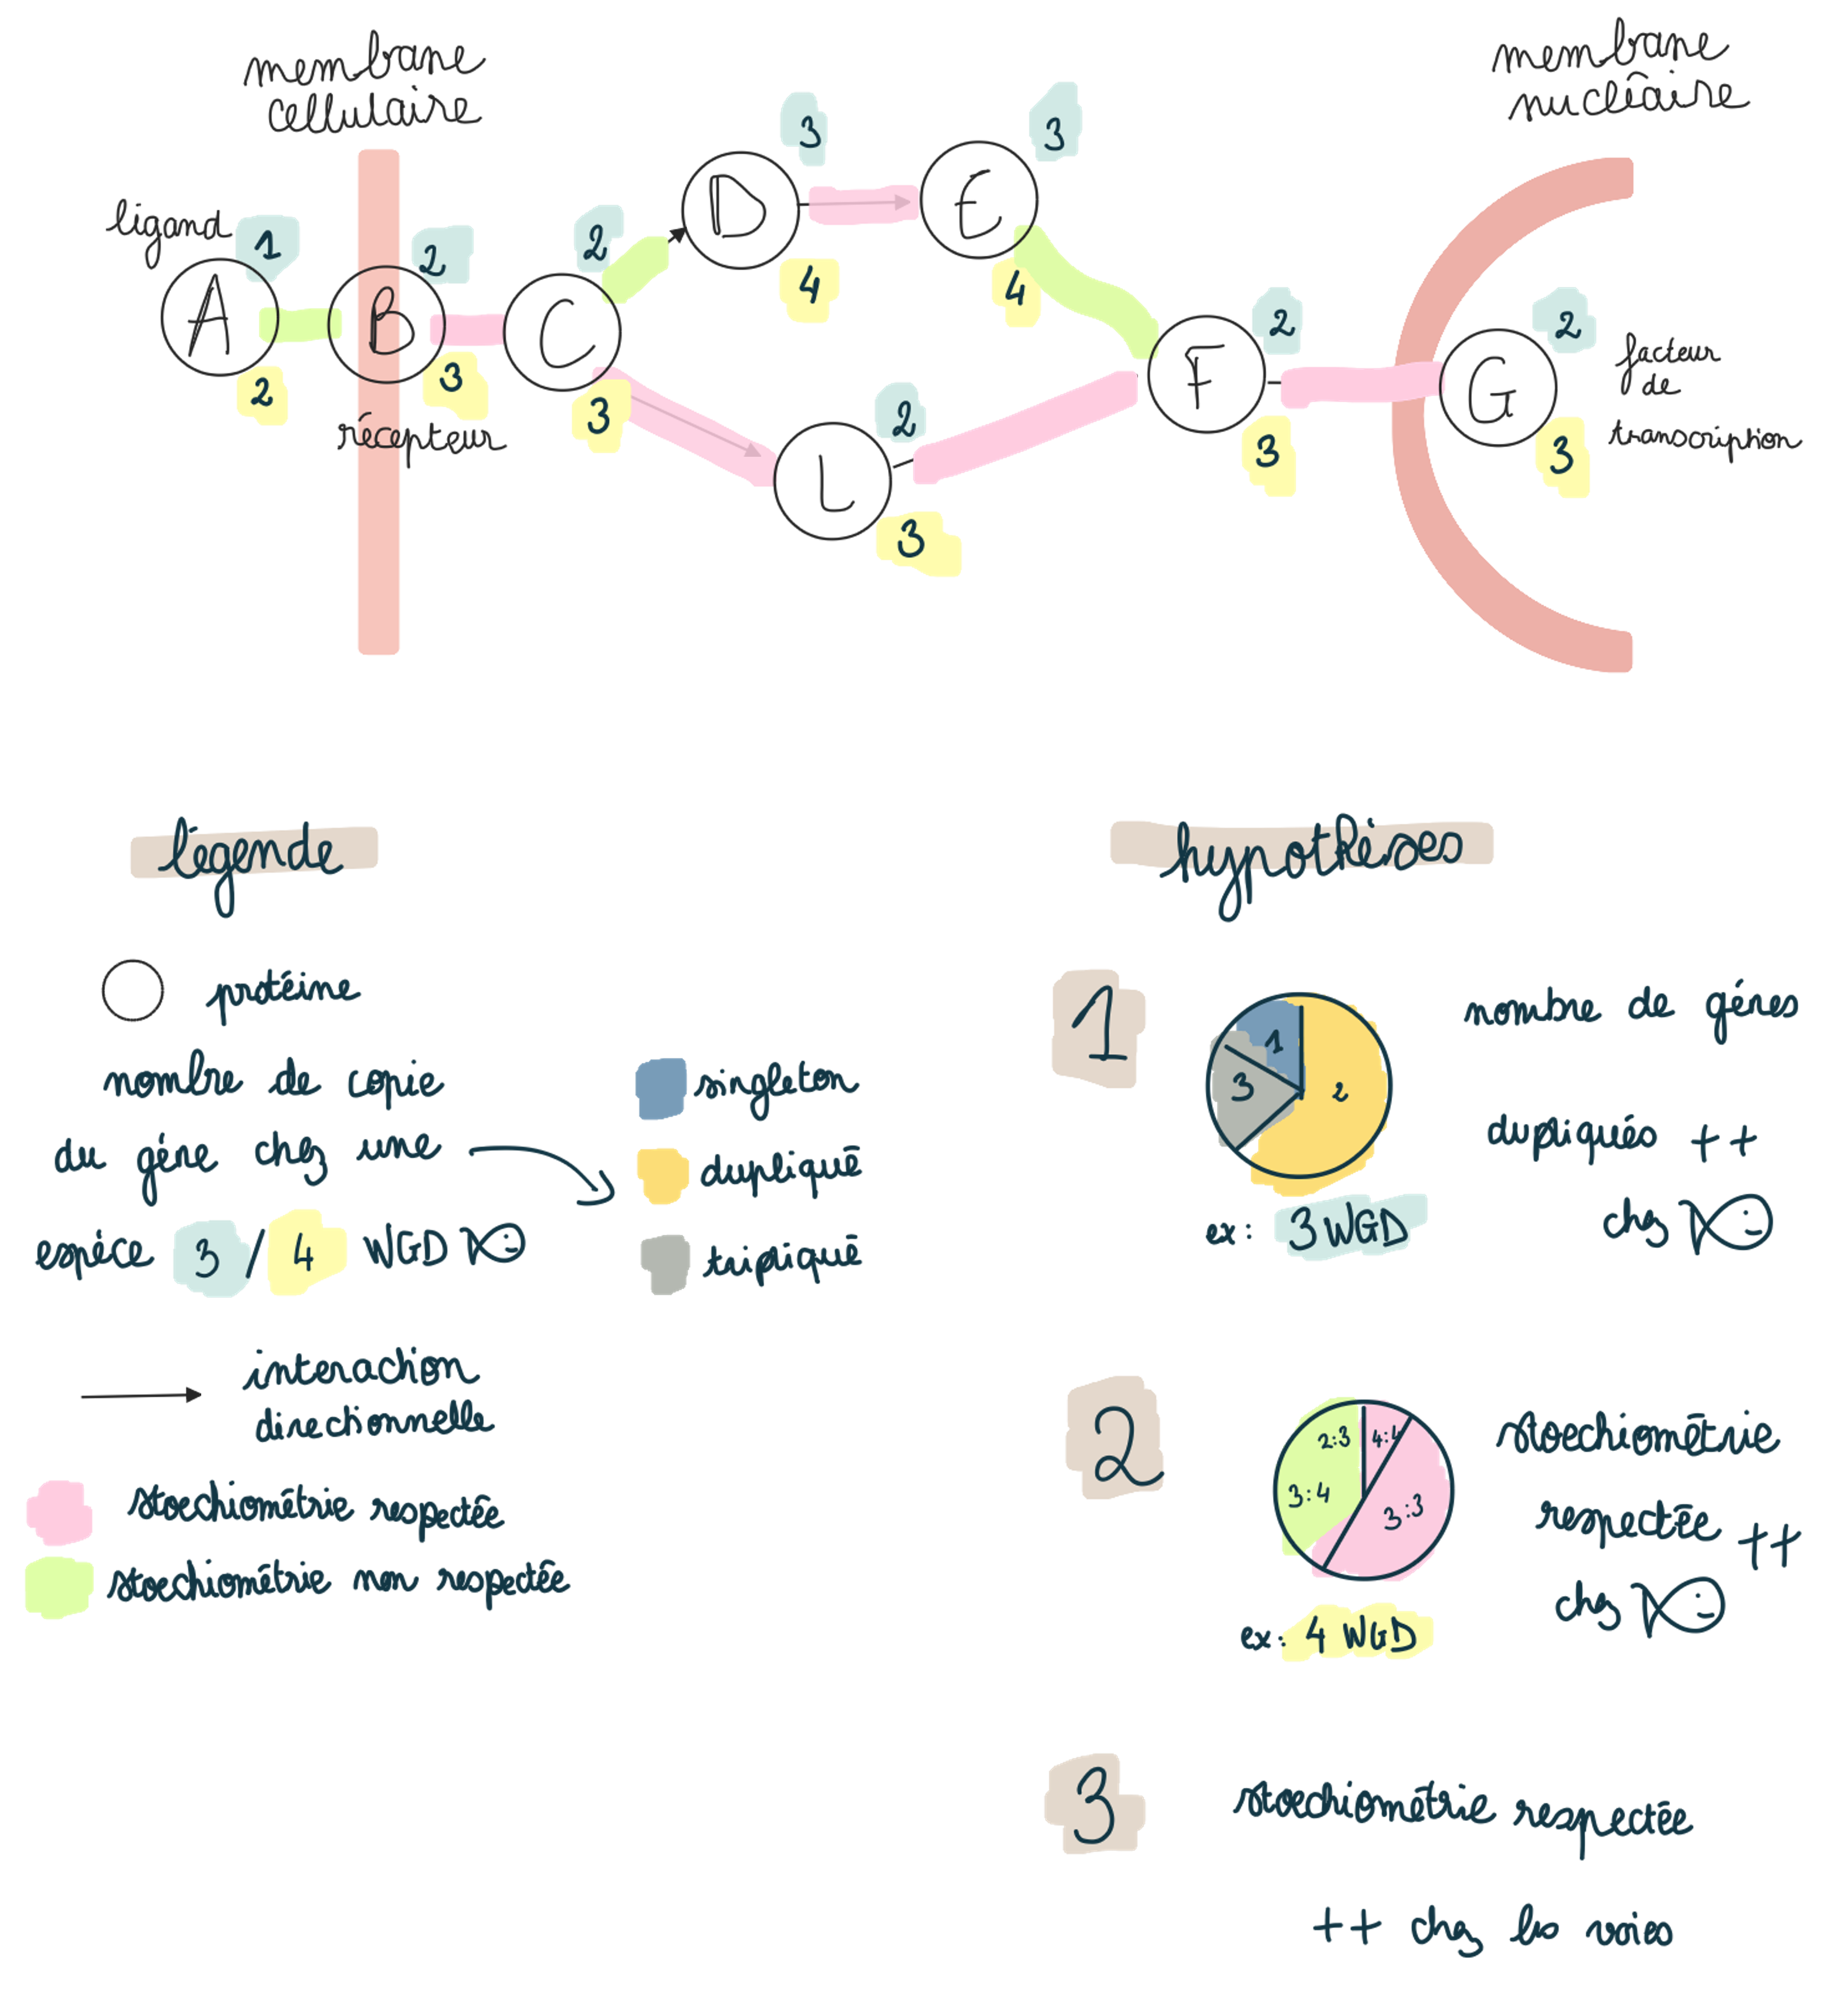
\includegraphics[width=1\textwidth]{figures/corps/figure15.png}
    \caption{Schéma récapitulatif de l'étude 2}
    \label{fig:15_schéma2}
\end{figure} 
\newpage

\section{Article}\label{art2}
\setlength{\headheight}{17.30428pt}
\addtolength{\topmargin}{-5.30428pt}
\includepdf[scale=0.9,pages=1-8,pagecommand={\thispagestyle{plain}}]{figures/articles/pico-2021.pdf}